\begin{frame}{Réseau de neurones non-récurrent}
    \begin{figure}
        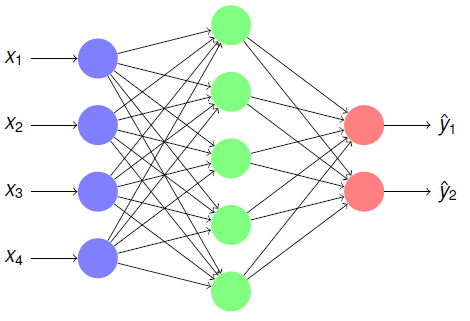
\includegraphics[height=.75\textheight,width=\textwidth,keepaspectratio]{images/arch_nn}
        \caption{Réseau de neurones feed-forward {\scriptsize\it -- Source : Cours R. \textsc{Hérault} \& P. \textsc{Leray}}}
    \end{figure}
    
\end{frame}


\begin{frame}{Architecture générale}
    \begin{figure}
        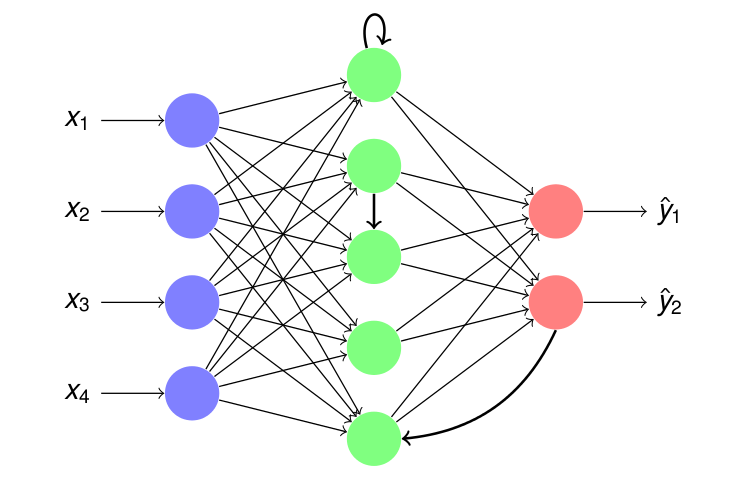
\includegraphics[height=.75\textheight,width=\textwidth,keepaspectratio]{images/arch_rnn_1}
        \caption{Réseau de neurones récurrent {\scriptsize\it -- Source : Cours R. \textsc{Hérault} \& P. \textsc{Leray}}}
    \end{figure}

\end{frame}

\begin{frame}{RNN d'Elman}
    \begin{figure}
        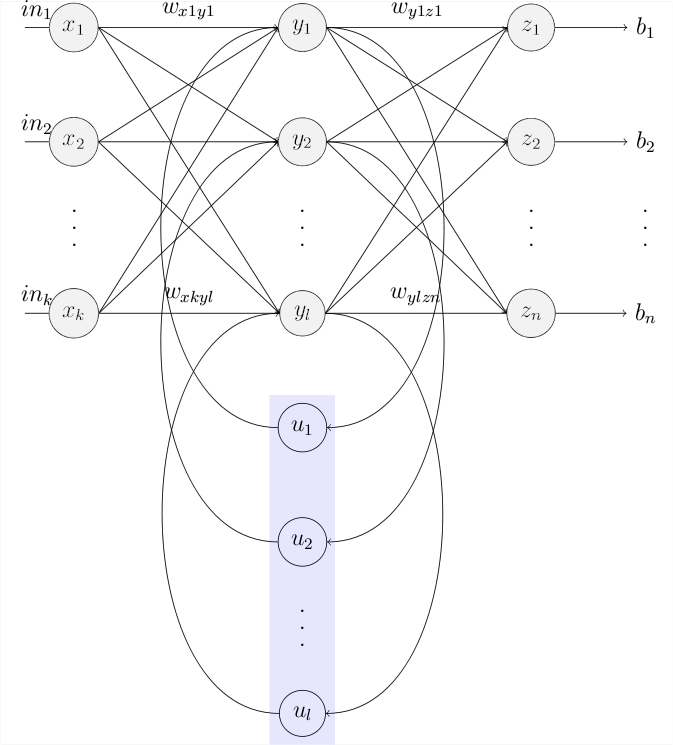
\includegraphics[height=.65\textheight,width=\textwidth,keepaspectratio]{images/Elman_srnn}
        \caption{RNN d'Elman {\scriptsize\it -- Source : wikimedia.org}}
    \end{figure}
    \vspace{-.5cm}
	\begin{itemize} 
		\item La couche $u_1 ... u_n$ sert de mémoire pour l'état précédent 
	\end{itemize}
\end{frame}

\begin{frame}{Echo State Networks}
    \begin{figure}
        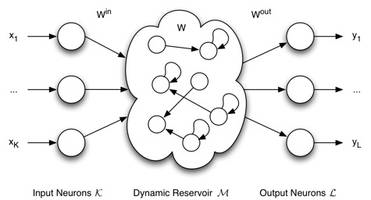
\includegraphics[height=.35\textheight,width=\textwidth,keepaspectratio]{images/echo}
        \caption{Echo State Network {\scriptsize\it -- Source : Université de Ulm}}
    \end{figure}
    \vspace{-.3cm}
    \begin{itemize} 
        \item Par \citeauthor{Jaeger01} en 2001 \cite{Jaeger01}
        \item Pas d'architecture précise
        \item Réservoir de neurones faiblement connectés aléatoirement entre eux \textit{(Reservoir computing)}
    \end{itemize}
\end{frame}


\begin{frame}{Liquid State Machines}
    \begin{figure}
        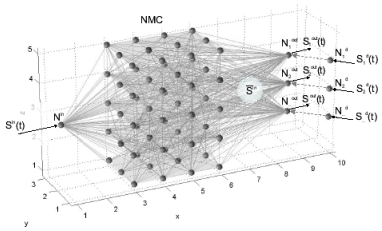
\includegraphics[height=.35\textheight,width=\textwidth,keepaspectratio]{images/liquid_state}
        \caption{Liquid State Machine {\scriptsize\it -- Source : F. \textsc{Ponulak}}}
    \end{figure}
    \vspace{-.3cm}
    \begin{itemize}
        \item Par \citeauthor{Maass02} en 2002 \cite{Maass02}
        \item Principe proche des \textit{Echo State Network}
        \item Réseau de neurones à décharge \textit{(spiking neural network)}
        \item Pas d'architecture précise
        \item Réservoir de neurones connectés aléatoirement entre eux
    \end{itemize}
\end{frame}

